\documentclass[11pt,a4paper]{article}

\usepackage[margin=2.5cm]{geometry}
\usepackage[T1]{fontenc}
\usepackage{lmodern}
\usepackage{microtype}
\usepackage{booktabs}
\usepackage{longtable}
\usepackage{xcolor}
\usepackage{listings}
\usepackage{amsmath}
\usepackage{enumitem}
\usepackage{graphicx}
\usepackage{tikz}
\usepackage[hidelinks]{hyperref}

\definecolor{codebg}{RGB}{247,247,247}
\definecolor{codekey}{RGB}{20,80,160}
\definecolor{codestr}{RGB}{150,60,20}
\definecolor{codecom}{RGB}{110,110,110}

\lstdefinestyle{json}{
  basicstyle=\ttfamily\footnotesize,
  backgroundcolor=\color{codebg},
  breaklines=true,
  breakatwhitespace=false,
  columns=fullflexible,
  keepspaces=true,
  showstringspaces=false,
  frame=single,
  framerule=0pt,
  framesep=6pt,
  xleftmargin=6pt,
  stringstyle=\color{codestr},
  literate=
    *{:}{{{\color{codekey}:}}}{1}
     {\{}{{{\color{codekey}\{}}}{1}
     {\}}{{{\color{codekey}\}}}}{1},
}

\lstdefinestyle{plain}{
  basicstyle=\ttfamily\footnotesize,
  backgroundcolor=\color{codebg},
  breaklines=true,
  columns=fullflexible,
  keepspaces=true,
  showstringspaces=false,
  frame=single,
  framerule=0pt,
  framesep=6pt,
  xleftmargin=6pt,
}

\lstset{style=json}

\newcommand{\code}[1]{\texttt{\small #1}}
\newcommand{\file}[1]{\texttt{\small #1}}
\newcommand{\menu}[1]{\textsf{#1}}

% ---- GitHub links to files in the repository ---------------------------------
\newcommand{\ghbase}{https://github.com/ArashMassoudieh/OpenHydroQual/blob/master}
\newcommand{\ghtree}{https://github.com/ArashMassoudieh/OpenHydroQual/tree/master}
\newcommand{\exfile}[1]{\href{\ghbase/#1}{\file{#1}}}
\newcommand{\exdir}[1]{\href{\ghtree/#1}{\file{#1}}}

% ---- Screenshot slots --------------------------------------------------------
% Drop a PNG with the given name into docs/figures/ and it is used automatically;
% until then a labelled placeholder box is drawn so the document still compiles.
\newcommand{\screenshot}[3][0.85]{%
  \begin{figure}[htbp]
  \centering
  \IfFileExists{figures/#2.png}
    {\includegraphics[width=#1\linewidth]{figures/#2}}
    {\fbox{\begin{minipage}[c][0.28\linewidth][c]{#1\linewidth}
       \centering\ttfamily\footnotesize\color{gray}
       [ screenshot placeholder ]\\[0.4em] figures/#2.png
     \end{minipage}}}
  \caption{#3}
  \label{fig:#2}
  \end{figure}}

\title{\textbf{A Layered Sedimentation Basin in OpenHydroQual}\\[0.3em]
       \large Building a four-layer settling column with four particle classes}
\author{}
\date{}

\begin{document}
\maketitle
\vspace{-2.5em}

\begin{abstract}
\noindent
This tutorial builds one complete model from scratch: a sedimentation basin
discretized into four settling layers, fed by a constant influent and drained by
an equal effluent, with \emph{no} underflow, and carrying four particle classes
of differing settling velocity. It is the model shipped as
\exdir{Examples/Sedimentation\_Basin\_Particle\_Classes}. Because nothing is
withdrawn from the floor, the only downward transport is gravity settling, and
the model reduces to a textbook result --- removal depends solely on the ratio
of settling velocity to overflow rate --- which makes it a good check that the
tool is doing what you think it is doing. Both routes are covered: the
graphical interface, and the equivalent model script. The final section compares
the simulated answer with the analytical one.
\end{abstract}

\tableofcontents

\section{What we are building}

\subsection{The physical system}

A rectangular or circular basin of plan area $A$ receives a flow $Q$ carrying
suspended solids. The same flow $Q$ leaves as clarified effluent from the top.
The basin is divided vertically into four completely mixed layers of equal
depth. Solids settle from each layer into the one below at a velocity $v_s$ that
depends on the particle class. Nothing is pumped out of the bottom, so solids
accumulate on the floor.

\begin{center}
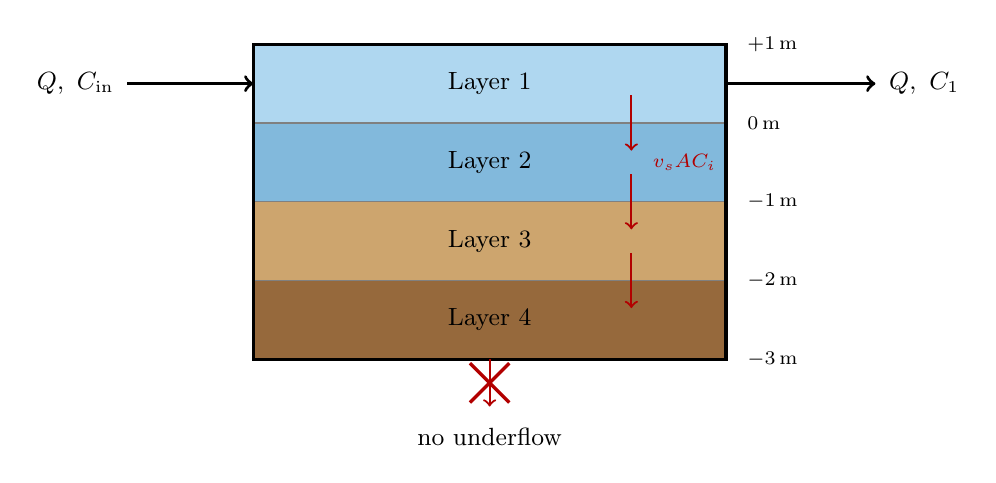
\begin{tikzpicture}[scale=1.0]
  \definecolor{l1}{RGB}{175,215,240}
  \definecolor{l2}{RGB}{130,185,220}
  \definecolor{l3}{RGB}{205,165,110}
  \definecolor{l4}{RGB}{150,105,60}
  \foreach \i/\c/\n in {0/l4/{Layer 4}, 1/l3/{Layer 3}, 2/l2/{Layer 2}, 3/l1/{Layer 1}} {
    \fill[\c] (0,\i) rectangle (6,\i+1);
    \draw[gray] (0,\i) rectangle (6,\i+1);
    \node[font=\small] at (3,\i+0.5) {\n};
  }
  \draw[very thick] (0,0) rectangle (6,4);
  % elevations
  \foreach \i/\z in {4/{$+1$}, 3/{$0$}, 2/{$-1$}, 1/{$-2$}, 0/{$-3$}}
    \node[font=\scriptsize, anchor=west] at (6.15,\i) {\z\,m};
  % influent / effluent
  \draw[->,very thick] (-1.6,3.5) -- (0,3.5);
  \node[font=\small,anchor=east] at (-1.65,3.5) {$Q,\ C_\mathrm{in}$};
  \draw[->,very thick] (6,3.5) -- (7.9,3.5);
  \node[font=\small,anchor=west] at (7.95,3.5) {$Q,\ C_1$};
  % settling arrows
  \foreach \i in {1,2,3} \draw[->,thick,red!70!black] (4.8,\i+0.35) -- (4.8,\i-0.35);
  \node[font=\scriptsize,red!70!black,anchor=west] at (4.95,2.5) {$v_sAC_i$};
  % no underflow
  \draw[->,thick,red!70!black] (3,0) -- (3,-0.6);
  \draw[very thick,red!70!black] (2.75,-0.05) -- (3.25,-0.55);
  \draw[very thick,red!70!black] (2.75,-0.55) -- (3.25,-0.05);
  \node[font=\small,anchor=north] at (3,-0.75) {no underflow};
\end{tikzpicture}
\end{center}

\subsection{Design point}

\begin{center}
\begin{tabular}{llr}
\toprule
Symbol & Quantity & Value \\
\midrule
$Q$            & Inflow $=$ outflow                & $2000$ m\textsuperscript{3}/day \\
$A$            & Plan area                          & $400$ m\textsuperscript{2} \\
$v^{*}=Q/A$    & \textbf{Overflow rate}             & $\mathbf{5}$ \textbf{m/day} \\
$z_0$          & Floor elevation                    & $-3$ m \\
$H$            & Depth of the basin                 & $4$ m \\
$V_\mathrm{tot}$ & Total initial volume             & $1600$ m\textsuperscript{3} \\
$C_\mathrm{in}$& Influent concentration, per class  & $50$ g/m\textsuperscript{3} \\
$Q_u$          & Underflow                          & $0$ \\
               & Simulated period                   & day $36526 \rightarrow 36556$ \\
\bottomrule
\end{tabular}
\end{center}

Only the floor elevation and the total depth are entered. The layer bottoms are
derived --- each layer is $H/4=1$ m thick, so they come out at $-3$, $-2$, $-1$
and $0$ m --- and the total volume is divided equally, giving
$400$~m\textsuperscript{3} per layer.

The four particle classes are chosen to straddle the overflow rate, so that
removal spans nearly the full range from negligible to almost complete:

\begin{center}
\begin{tabular}{lrrr}
\toprule
Class & $v_s$ (m/day) & $v_s/v^{*}$ & Expected removal \\
\midrule
\code{P1} & $0.5$ & $0.1$ & $9.1\%$ \\
\code{P2} & $2$   & $0.4$ & $28.6\%$ \\
\code{P3} & $10$  & $2$   & $66.7\%$ \\
\code{P4} & $50$  & $10$  & $90.9\%$ \\
\bottomrule
\end{tabular}
\end{center}

\subsection{Components used}

\begin{center}
\begin{tabular}{lll}
\toprule
Role & Type & Plugin file \\
\midrule
Particle classes      & \code{Particle}                & \file{main\_components.json} \\
Influent boundary     & \code{Reactor}                 & \file{mass\_transfer.json} \\
The basin             & \code{Clarifier (4 layers)}    & \file{wastewater.json} \\
Effluent boundary     & \code{fixed\_head}             & \file{main\_components.json} \\
Influent connection   & \code{Fixed flow}              & \file{wastewater.json} \\
Effluent connection   & \code{Effluent flow}           & \file{wastewater.json} \\
\bottomrule
\end{tabular}
\end{center}

\code{Clarifier (4 layers)} is a \emph{composite}: dropping one on the diagram
creates four \code{Settling compartment} blocks and the three
\code{Sedimentation tank element interface} links between them, all driven by
the composite's own properties. See \exfile{docs/composite\_blocks.tex} for how
composite types are declared.

\section{Route A --- building it in the graphical interface}

\subsection{Start a project and load the plugins}

\begin{enumerate}[leftmargin=1.4em]
\item \menu{File $\rightarrow$ New Project}. \file{main\_components.json} is
      loaded automatically; the other two must be added.
\item \menu{File $\rightarrow$ Preferences $\rightarrow$ Add plugin} opens the
      \menu{Select Plugin} dialog, which lists the plugins that ship with
      OpenHydroQual. Choose \menu{Mass Transfer} and press \menu{OK}.
\item Open the same dialog again and choose \menu{Wastewater processes}.
\end{enumerate}

Both plugins are in the shipped list, so there is no need to hunt for the files
on disk. Each entry in the dialog loads exactly one plugin file --- \menu{Mass
Transfer} loads \file{mass\_transfer.json} and \menu{Wastewater processes} loads
\file{wastewater.json} --- which is why the dialog is opened twice.
(\menu{File $\rightarrow$ Preferences $\rightarrow$ Add plugin from file} does the
same job through a file browser, and is only needed for a plugin you wrote
yourself and that is not in the list.)

The \menu{Add Objects} menu and the toolbars rebuild themselves each time a
plugin is added. Menu entries show each type's \emph{description}, not its type
name --- so the basin appears as \menu{Clarifier: sedimentation basin
discretized into four settling layers}, and composites are listed after a
separator at the bottom of \menu{Add Objects $\rightarrow$ Blocks}.

\screenshot[0.75]{01-add-plugin}{The \menu{Select Plugin} dialog, reached through
\menu{File $\rightarrow$ Preferences $\rightarrow$ Add plugin}, with
\menu{Wastewater processes} selected. \menu{Mass Transfer} is loaded the same
way.}

\subsection{Declare the four particle classes}

Constituents must exist \emph{before} the blocks, so that every block picks up
the per-constituent properties.

\begin{enumerate}[leftmargin=1.4em]
\item \menu{Add Objects $\rightarrow$ Chemistry $\rightarrow$ Solid Particle}.
\item In the property panel set \menu{Name} to \code{P1} and
      \menu{Settling velocity} to \code{0.5} m/day.
\item Repeat three more times for \code{P2}, \code{P3} and \code{P4} with
      $2$, $10$ and $50$ m/day.
\end{enumerate}

Leave \menu{Turbidity Coefficient} and \menu{Turbidity Exponent} at zero; they
only affect the reported \code{turbidity} output.

\screenshot[0.42]{02-particle-properties}{The four particle classes under
\menu{Constituents} in the Object Browser, with \code{P1} selected and its
settling velocity set to $0.5$ m/day.}

\subsection{Place the influent boundary}

\begin{enumerate}[leftmargin=1.4em]
\item \menu{Add Objects $\rightarrow$ Blocks $\rightarrow$ Reactor}, and click on
      the canvas to place it.
\item Set the properties in Table~\ref{tab:influent}.
\end{enumerate}

\begin{table}[htbp]
\centering
\caption{Properties of the \code{Influent} reactor.}
\label{tab:influent}
\begin{tabular}{llr}
\toprule
Property & Meaning & Value \\
\midrule
\menu{Name}                     & --                                & \code{Influent} \\
\menu{Initial Storage}          & working volume                    & $200$ m\textsuperscript{3} \\
\menu{Bottom elevation}         & --                                & $0$ m \\
\menu{Constant inflow}          & external feed                     & $2000$ m\textsuperscript{3}/day \\
\menu{P1..P4 Concentration}     & initial condition                 & $50$ g/m\textsuperscript{3} each \\
\menu{P1..P4 Constant Inflow concentration} & feed strength         & $50$ g/m\textsuperscript{3} each \\
\bottomrule
\end{tabular}
\end{table}

This block is a boundary condition, not part of the basin. It receives
$2000$~m\textsuperscript{3}/day of water at $50$~g/m\textsuperscript{3} per
class and passes the same flow on, so it holds a constant concentration and acts
as an inexhaustible source. Setting both the initial \emph{and} the inflow
concentration to $50$ starts it at steady state, avoiding a startup transient.

\subsection{Place the basin}

\menu{Add Objects $\rightarrow$ Blocks}, then the entry
\menu{Clarifier: sedimentation basin discretized into four settling layers}
below the separator. One click creates the whole four-layer stack. Set:

\begin{table}[htbp]
\centering
\caption{Properties of the \code{Sed\_Basin} composite. This handful of values
describes the whole four-layer stack; the per-layer geometry is derived from
them. The two optional time-series inputs, \menu{External inflow time series
into the top layer} and \menu{Time variable component of the underflow}, are
left empty here.}
\label{tab:basin}
\begin{tabular}{llr}
\toprule
Property & Meaning & Value \\
\midrule
\menu{Name} & -- & \code{Sed\_Basin} \\
\menu{Cross-sectional area of the layer interfaces} & $A$ & $400$ m\textsuperscript{2} \\
\menu{Flow drawn downward through the layers}       & $Q_u$ & $\mathbf{0}$ \\
\menu{Elevation of the clarifier floor}             & $z_0$ & $-3$ m \\
\menu{Depth of the clarifier}                       & $H$ & $4$ m \\
\menu{Initial volume of water in the clarifier}     & $V_\mathrm{tot}$ & $1600$ m\textsuperscript{3} \\
\bottomrule
\end{tabular}
\end{table}

Three points deserve emphasis.

\begin{description}[style=nextline,leftmargin=1.2em]
\item[The underflow is what makes this a settling column rather than a clarifier.]
Setting \menu{Flow drawn downward through the layers} to zero puts zero
advective flow on all three internal interfaces at once. The only remaining
downward transport is settling.

\item[The layer geometry is derived, not entered.]
The four layers are equal quarters of the depth, so their bottom elevations
follow from the floor and the depth alone:
\begin{equation}
z_4 = z_0, \qquad z_3 = z_0 + \tfrac{H}{4}, \qquad
z_2 = z_0 + \tfrac{H}{2}, \qquad z_1 = z_0 + \tfrac{3H}{4},
\end{equation}
which for this design point gives $-3$, $-2$, $-1$ and $0$ m. Likewise
$V_\mathrm{tot}$ is split four ways, giving $400$~m\textsuperscript{3} per
layer. This is what keeps the stack self-consistent: because the elevations are
generated rather than typed, they are always strictly decreasing downward, and
the settling gate of Section~\ref{sec:physics} can never be accidentally closed.

\item[Volume and depth are independent.]
$V_\mathrm{tot}$ is an \emph{initial condition} --- how much water is in the
basin at $t=0$ --- while $H$ and $A$ describe the vessel. For a full prismatic
basin they agree, $V_\mathrm{tot}=A\,H=1600$~m\textsuperscript{3}, as here, but
nothing forces that.
\end{description}

\screenshot[0.85]{03-basin-properties}{The property panel of the
\code{Clarifier (4 layers)} composite. Every value of Table~\ref{tab:basin} is
visible at once --- note \menu{Depth of the clarifier} and
\menu{Elevation of the clarifier floor} in place of four separate layer
elevations, \menu{Initial volume of water in the clarifier} in place of four
layer volumes, and \menu{Flow drawn downward through the layers} $=0$. There is
no per-layer entry anywhere in the panel: that geometry is derived. The
\code{P4:\ldots} rows at the top are the per-constituent properties, which stay
at zero --- the basin starts clean.}

\subsection{Place the effluent boundary}

\menu{Add Objects $\rightarrow$ Blocks $\rightarrow$ Fixed-head boundary}. Name it
\code{Effluent}, set \menu{Storage} to $100000$, \menu{Bottom elevation} to $0$
and \menu{head} to $0$. It is a receiving water body large enough not to matter.

\subsection{Draw the two links}

Link types are toggles: pick the type, then drag from the source block to the
destination block.

\begin{enumerate}[leftmargin=1.4em]
\item \menu{Add Objects $\rightarrow$ Links $\rightarrow$ Fixed flow}. Drag from
      \code{Influent} to \code{Sed\_Basin}. Name it \code{Influent to Basin} and
      set \menu{Flow rate} to $2000$ m\textsuperscript{3}/day.
\item \menu{Add Objects $\rightarrow$ Links $\rightarrow$ Effluent flow (clarified
      water drawn from the top of a clarifier)}. Drag from \code{Sed\_Basin} to
      \code{Effluent}. Name it \code{Basin to Effluent} and set \menu{Flow rate}
      to $2000$ m\textsuperscript{3}/day --- the \emph{same} number.
\end{enumerate}

You never pick a layer. The composite resolves the endpoint itself from its
\code{external\_links} table: the wildcard entry sends any unlisted link type to
layer~1, and \code{Effluent flow} is mapped explicitly to layer~1 as well. Had
you attached a \code{Sludge flow} link, it would have landed on layer~4 --- which
is exactly what we are \emph{not} doing here.

\screenshot[0.98]{04-diagram}{The finished diagram: three nodes and two links.
The four layers live inside the single \code{Clarifier (4 layers)} node.}

\subsection{Simulation settings}

Open \menu{View $\rightarrow$ Object Browser}, expand \menu{Settings} and select
\menu{general\_parameters}:

\begin{itemize}[leftmargin=1.4em]
\item \menu{Simulation start time} $=36526$
\item \menu{Simulation end time} $=36556$ (30 days)
\item \menu{Output File Name (All outputs)} $=$ \file{output.txt}
\end{itemize}

The defaults under \menu{solver\_settings} are fine; this model is small, linear
in the constituents, and converges without tuning.

\subsection{Validate, run, save}

\menu{Model $\rightarrow$ Validate}, then \menu{Model $\rightarrow$ Run}. Then
\menu{File $\rightarrow$ Save as} to write the \file{.ohq} model script.

\subsection{Viewing results}
\label{sec:viewing}

The engine never simulates a composite --- it simulates the members --- so the
results live on the layers, and the basin's context menu groups them one
submenu per member. Right-click the basin on the diagram and follow

\begin{center}
\menu{Results} $\rightarrow$ \menu{Layer1} $\rightarrow$ \menu{P1:Concentration}
\end{center}

\noindent
to plot the effluent concentration of the first particle class. The member
submenus are labelled by role --- \menu{Layer1} through \menu{Layer4} --- rather
than by the instance-qualified names (\code{Sed\_Basin\_\_Layer1}) that appear in
\file{output.txt}. Walking the same menu with a different layer or a different
class gives every combination:

\begin{itemize}[leftmargin=1.4em]
\item \menu{Layer1} $\rightarrow$ \menu{P\emph{n}:Concentration} is the effluent
      quality for class $n$. It should settle at the value in
      Section~\ref{sec:verify}.
\item \menu{Layer2} and \menu{Layer3} plotted for the same class should level off
      at the \emph{same} value as layer~1 --- the middle layers convey rather
      than accumulate.
\item \menu{Layer4} $\rightarrow$ \menu{P\emph{n}:Concentration} rises linearly
      and never levels off. That is the sludge blanket, and it is the expected
      behaviour of a basin that is never desludged.
\end{itemize}

The three internal interfaces are on the same menu, below the layers. They are
worth a look:

\begin{itemize}[leftmargin=1.4em]
\item \menu{interface12} $\rightarrow$ \menu{Flow rate} should be flat zero,
      which is the direct confirmation that there is no underflow.
\item \menu{interface12} $\rightarrow$ \menu{P\emph{n}:Settling transfer rate}
      is the settling flux in g/day. Compared against the same quantity on
      \menu{interface34}, the two converge to the same number once steady --- the
      conveyor again.
\end{itemize}

If a plot looks blank or flat at an implausible value, check the axis range
before suspecting the model: the plot window keeps whatever zoom it was last
given, and a series can sit entirely outside the visible region.

\section{Route B --- the model script}

An \file{.ohq} file is a plain-text command script, so the whole model can be
written by hand. The listing below is complete and runnable; it produces the
results in Section~\ref{sec:verify}. Values carry no unit suffix, which means
they are in the engine's base units --- metres, grams and \emph{days}.

\begin{lstlisting}[style=plain]
loadtemplate; filename = <path>/resources/main_components.json
addtemplate;  filename = <path>/resources/mass_transfer.json
addtemplate;  filename = <path>/resources/wastewater.json

setvalue; object=system, quantity=simulation_start_time, value=36526
setvalue; object=system, quantity=simulation_end_time,   value=36556
setvalue; object=system, quantity=alloutputfile,         value=output.txt

create constituent;type=Particle,name=P1,settling_velocity=0.5
create constituent;type=Particle,name=P2,settling_velocity=2
create constituent;type=Particle,name=P3,settling_velocity=10
create constituent;type=Particle,name=P4,settling_velocity=50

create block;type=Reactor,name=Influent,Storage=200,bottom_elevation=0,
    constant_inflow=2000,
    P1:concentration=50,P2:concentration=50,
    P3:concentration=50,P4:concentration=50,
    P1:constant_inflow_concentration=50,P2:constant_inflow_concentration=50,
    P3:constant_inflow_concentration=50,P4:constant_inflow_concentration=50,
    x=0,y=900

create composite;type=Clarifier (4 layers),name=Sed_Basin,
    surface_area=400,underflow=0,
    floor_elevation=-3,depth=4,total_volume=1600,
    x=700,y=900

create block;type=fixed_head,name=Effluent,Storage=100000,
    bottom_elevation=0,head=0,x=1400,y=900

create link;from=Influent,to=Sed_Basin,type=Fixed flow,
    flow=2000,name=Influent to Basin
create link;from=Sed_Basin,to=Effluent,type=Effluent flow,
    flow=2000,name=Basin to Effluent
\end{lstlisting}

\noindent
Each \code{create} command must occupy a single line --- the line breaks above
are for the page only. A few rules the parser enforces:

\begin{itemize}[leftmargin=1.4em]
\item Commands run in order, and \code{create constituent} must precede the
      blocks, otherwise the blocks never acquire \code{P1:\ldots} properties.
\item Type names may contain spaces and parentheses
      (\code{Clarifier (4 layers)}); only \code{;}, \code{,} and \code{=} are
      structural.
\item A value may carry an explicit unit in brackets, as
      \code{settling\_velocity=0.5[m/day]}. Without brackets the value is
      interpreted in base units, which for a velocity is m/day.
\item Whitespace around \code{=} and \code{,} is trimmed.
\end{itemize}

What the interface saves is the same script with every property written out
explicitly, including defaults --- see
\exfile{Examples/Sedimentation\_Basin\_Particle\_Classes/Sedimentation\_Basin\_Particle\_Classes.ohq}.

\section{What the model actually computes}
\label{sec:physics}

\subsection{Mass transfer across a link}

Every \code{Particle} contributes a \code{masstransfer} expression to each link:

\begin{lstlisting}
"masstransfer": "_ups(flow;concentration)
   + settling_velocity*area*( _hsd(bottom_elevation.s-bottom_elevation.e-1e-7)*concentration.s
                            - _hsd(bottom_elevation.e-bottom_elevation.s-1e-6)*concentration.e )"
\end{lstlisting}

The first term is ordinary advection, upstream-weighted. The second is settling:
\code{\_hsd} is a Heaviside step, so the term is active only in the direction of
decreasing bottom elevation, and \code{area} is the interface area. For an
interface link between layer $i$ (above) and layer $i+1$ (below) this is simply

\begin{equation}
J_{i \rightarrow i+1} \;=\; v_s\, A\, C_i .
\end{equation}

This is also why the \code{Fixed flow}, \code{Effluent flow} and
\code{Sludge flow} link types declare an \code{area} of $10^{-9}$: they are
plumbing, and must not settle anything.

\subsection{Steady state}

With $Q_u=0$, only layer~1 has throughflow. Its mass balance at steady state is

\begin{equation}
Q\,C_\mathrm{in} \;=\; \underbrace{Q\,C_1}_{\text{effluent}} \;+\; \underbrace{v_s A\, C_1}_{\text{settled}}
\qquad\Longrightarrow\qquad
\boxed{\;C_1 \;=\; \frac{C_\mathrm{in}}{1 + v_s A/Q}\;}
\end{equation}

so the removal efficiency depends on nothing but the ratio of settling velocity
to overflow rate $v^{*}=Q/A$:

\begin{equation}
\eta \;=\; 1-\frac{C_1}{C_\mathrm{in}} \;=\; \frac{v_s/v^{*}}{1+v_s/v^{*}} .
\end{equation}

Layers 2 and 3 receive $v_sAC_{i-1}$ and pass on $v_sAC_i$, so at steady state
$C_2=C_3=C_1$: they are a conveyor, not a sink. Layer~4 has an inlet and no
outlet, so it accumulates at a constant rate and its concentration grows
linearly,

\begin{equation}
C_4(t) \;=\; \frac{Q\,C_\mathrm{in}\,\eta}{V}\; t ,
\end{equation}

which is the sludge blanket. This is the physically correct behaviour of a basin
that is never desludged, and it is the one quantity in the model that never
reaches steady state.

\section{Verification}
\label{sec:verify}

Running the script above for 30 days and reading
\code{Sed\_Basin\_\_Layer1\_P\emph{n}:concentration} from \file{output.txt}
reproduces the analytical solution to five significant figures:

\begin{center}
\begin{tabular}{lrrrrr}
\toprule
Class & $v_s$ (m/day) & $C_1$ simulated & $C_1$ analytical & $C_4$ at day 30 & Removal \\
\midrule
\code{P1} & $0.5$ & $45.4545$ & $45.4545$ & $609$  & $9.1\%$ \\
\code{P2} & $2$   & $35.7143$ & $35.7143$ & $2131$ & $28.6\%$ \\
\code{P3} & $10$  & $16.6667$ & $16.6667$ & $5119$ & $66.7\%$ \\
\code{P4} & $50$  & $4.5454$  & $4.5455$  & $7028$ & $90.9\%$ \\
\bottomrule
\end{tabular}
\end{center}

Three further checks are worth running on any model of this kind:

\begin{itemize}[leftmargin=1.4em]
\item $C_2$ and $C_3$ equal $C_1$, confirming the middle layers are conveying
      rather than accumulating.
\item The interface flows \code{Sed\_Basin\_\_interface12\_flow} and its two
      siblings are exactly zero, confirming there is no underflow.
\item Mass balance closes on each class. For \code{P3}: $100\,000$ g/day in
      $=33\,333$ g/day out $+\ 66\,667$ g/day settled.
\end{itemize}

\section{Pitfalls}

\begin{description}[style=nextline,leftmargin=1.2em]

\item[Read layer 1, not the effluent block.]
Effluent quality is \code{Sed\_Basin\_\_Layer1\_P\emph{n}:concentration}. The
column \code{Effluent\_P\emph{n}:concentration} is the concentration inside the
$100\,000$~m\textsuperscript{3} receiving reservoir, which is still filling and
is much lower. This trips people up on the first run.

\item[Equal elevations silently disable settling.]
The settling term is gated on $z_i > z_{i+1}$: give two adjacent layers the same
bottom elevation and solids simply stop moving, with no diagnostic. The
\code{Clarifier (4 layers)} composite forecloses this by deriving the elevations
from the floor and the depth, but the trap is live in any stack assembled from
bare \code{Settling compartment} blocks --- including one produced by
\menu{Ungroup}. If such a model shows zero removal, check the elevations first.

\item[Constituents before blocks.]
In a hand-written script, a \code{create block} that precedes
\code{create constituent} produces a block with no particle properties, and the
\code{P\emph{n}:\ldots} assignments are silently dropped.

\item[Watch the log for missing-property errors.]
Messages of the form \code{property 'X' does not exist in 'Y'} mean an
expression referenced a quantity that is not there, and the expression quietly
evaluated to zero. They look like noise and are not. The one remaining message
in this model, \code{property 'inflow' does not exist in 'Effluent'}, is benign
--- a \code{fixed\_head} boundary has no inflow term, so its loading is
correctly zero.

\item[The console executable needs composite support compiled in.]
\file{terminal/TOpenHydroQual/} must include \file{Composite.cpp}, otherwise
\code{create composite} is ignored and the run fails with
\code{Block 'Sed\_Basin' does not exist!}.

\end{description}

\section{Variations to try}

\begin{itemize}[leftmargin=1.4em]
\item \textbf{Turn it into a real clarifier.} Attach a \code{Sludge flow} link
      from the basin to a waste boundary and set \menu{Flow drawn downward
      through the layers} to that rate. The link lands on layer~4 automatically,
      and layer~4 reaches a steady sludge blanket instead of accumulating.
\item \textbf{Change the overflow rate.} Halving \menu{Cross-sectional area of
      the layer interfaces} to $200$~m\textsuperscript{2} doubles $v^{*}$ to
      $10$~m/day and pushes every class's removal down; the tabulated $\eta$
      values move to $4.8$, $16.7$, $50$ and $83.3\%$.
\item \textbf{Deepen the basin.} Raise \menu{Depth of the clarifier} on its own
      and the four layer elevations move together, staying evenly spaced.
      Steady-state removal does not budge --- it depends on $Q/A$, not on depth
      --- but the transient does, through the layer volumes.
\item \textbf{Refine the discretization.} Compare against the two-compartment
      \code{Clarifier}. With no underflow the steady-state effluent is identical
      --- it depends only on layer~1 --- but the sludge blanket and the transient
      differ. Note that the two-compartment type still takes its interface and
      floor elevations individually; only \code{Clarifier (4 layers)} derives
      them.
\item \textbf{Use a measured distribution.} Replace the four classes with a
      settling-velocity distribution from a column test; the model structure is
      unchanged.
\end{itemize}

\end{document}
